\documentclass[letterpaper]{article}
% Used to do math and such (I think...)
\usepackage{amsmath}
\usepackage{amssymb}

% Used to color text (for todos)
\usepackage{xcolor}

% Used to embed pdfs from yEd and other sources
\usepackage{graphicx}

% Used to embed gnuplot output into document
\usepackage{epstopdf}

% Used to have a table span multiple pages.
\usepackage{longtable}

\usepackage{pdflscape}
\usepackage{geometry}

\usepackage{listingsutf8}
\usepackage{array}
\usepackage{multicol}
\usepackage{multirow}

\usepackage{algorithm}
\usepackage{algpseudocode}

\usepackage{float}

\usepackage{xspace}

\usepackage{subfig}
\usepackage{wrapfig}

% Deal with backwards quotes because evidently Latex doesn't know better.
\usepackage [english]{babel}
\usepackage [autostyle, english = american]{csquotes}
\MakeOuterQuote{"}

\usepackage{mathrsfs}

\DeclareMathOperator{\trace}{Tr}
\DeclareMathOperator{\argmax}{argmax}

\newcommand{\Erdos}{Erd\H{o}s\xspace}
\newcommand{\Renyi}{R\'enyi\xspace}
\newcommand{\Prob}[1]{\mathbb{P}\left( #1 \right)}
\newcommand{\Expected}[1]{\mathbb{E}\left( #1 \right)}

\newcommand{\Derivative}[1]{ \frac{d}{d #1} }
\newcommand{\NDerivative}[2]{ \frac{d^{#2}}{d #1^{#2}}}
\newcommand{\PartialDer}[1]{ \frac{\partial}{\partial #1} }
\newcommand{\NPartialDer}[2]{ \frac{\partial^{#2}}{\partial #1^{#2}} }

\newcommand{\NetworksEq}[2]{Eq. (#1) p. #2 of \textit{Networks} }
\newcommand{\NetworksFig}[2]{Fig. (#1) p. #2 of \textit{Networks} }
\newcommand{\NetworksSec}[2]{\S #1 p. #2 of \textit{Networks}}

\newcommand{\Floor}[1]{\left \lfloor #1 \right \rfloor}

\newcommand{\TODO}[1]{\textcolor{red}{#1}}

\newgeometry{margin=1.125in}

\begin{document}

\title{CSCI-5622: When They Buzz}
\author{Alex Gendreau \and Garrett Lewellen \and Tyler Behm}
\date{May 7\textsuperscript{th}, 2015}

\maketitle

\section*{Problem}

\paragraph{} Contestants in a quiz bowl may answer a question as it is being read by buzzing in. We wish to predict when this will happen so that an artificial agent will buzz in just before other contestants. We treat this as two separate problems 1) at what point in the question will the user buzz in, and 2) will user answer correctly. Correctly answered positions will be reported with a positive sign, and incorrectly negatively. We measure (1) by root mean square error (RMSE) and (2) by sign accuracy (ACC).

\section*{Original Approach}

\paragraph{} We originally proposed a user-dependent probabilistic model based on independence assumptions to pick the position with the highest probability given question features. Using logistic regression we found the approach slow and inaccurate (RMSE 106). We pivoted in favor of two simpler parallel lines of work: the Expected Value approach and Right-Wrong approach.

\section*{Expected Value Approach}

\begin{figure}[H]
	\begin{center}
		\resizebox{0.8\linewidth}{!}{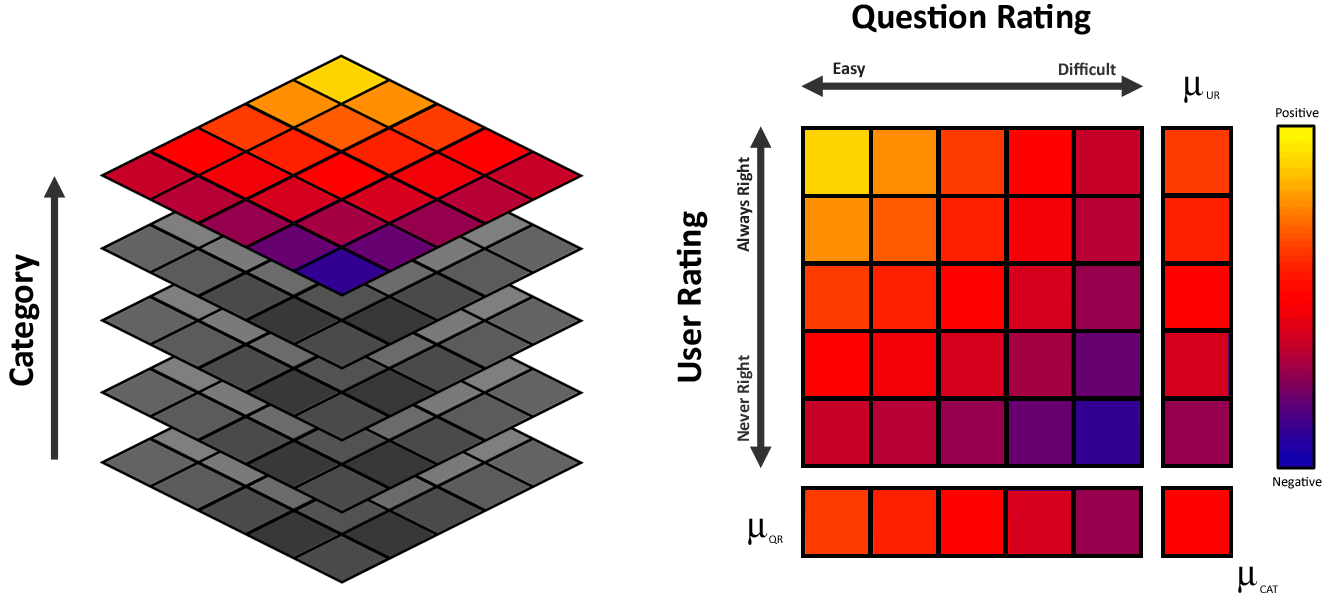
\includegraphics{expectedModel.png}}
	\end{center}
	\caption{Visual representation of the approach. If user rating or question rating are unknown, then expected positions $\mu_{QR}$ and $\mu_{UR}$ are used, or $\mu_{CAT}$ if neither is known.}
	\label{fig:expectedValue}
\end{figure}

\paragraph{} Garrett's simplest approach reported the expected position based on category, user rating, and question rating as depicted in Fig. (\ref{fig:expectedValue}). Users' abilities are measured by the portion of questions they answer correctly denoted by an integer value in $[-7, 7]$. Questions' difficulties are similar, but measured by portion of users who answer them correctly denoted by an integer in $[-2, 2]$. Garrett believed these features ultimately influenced the resulting sign and position. Result: RMSE of 87.48 and ACC of 72.50\%.

\begin{figure}[H]
	\begin{center}
		\resizebox{0.7\linewidth}{!}{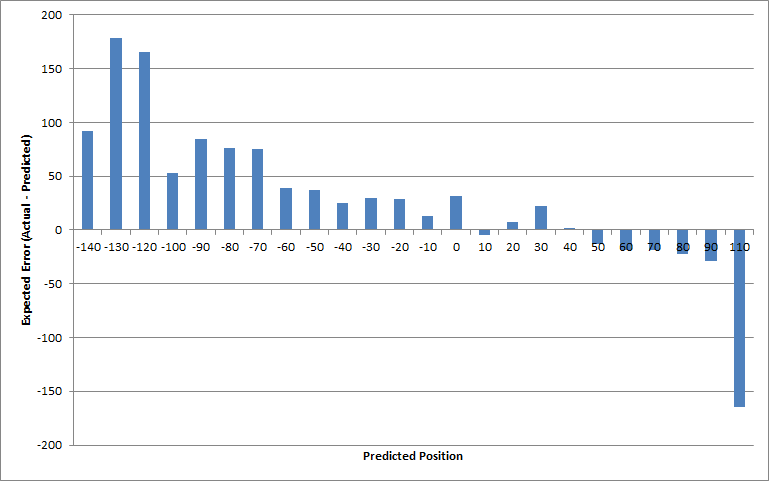
\includegraphics{expectedModelErrorAnalysis.png}}
	\end{center}
	\caption{Expected error as a function of predicted value.}
	\label{fig:expectedValue:errorAnalysis}
\end{figure}

\paragraph{} To improve RMSE, Garrett looked at the relationship between expected error and predicted position. Applying these error corrections to subsequent predictions produced RMSE of 84.39 and ACC of 73.02\%. Repeating the process three more times yielded RMSE of 83.73 and 72.65\%. Next, he looked at the most frequently reported position, user rating, and question rating to apply further adjustments based on category to obtain RMSE of 83.25 and sign accuracy of 73.5\%.

\begin{figure}[H]
	\begin{center}
		\resizebox{\linewidth}{!}{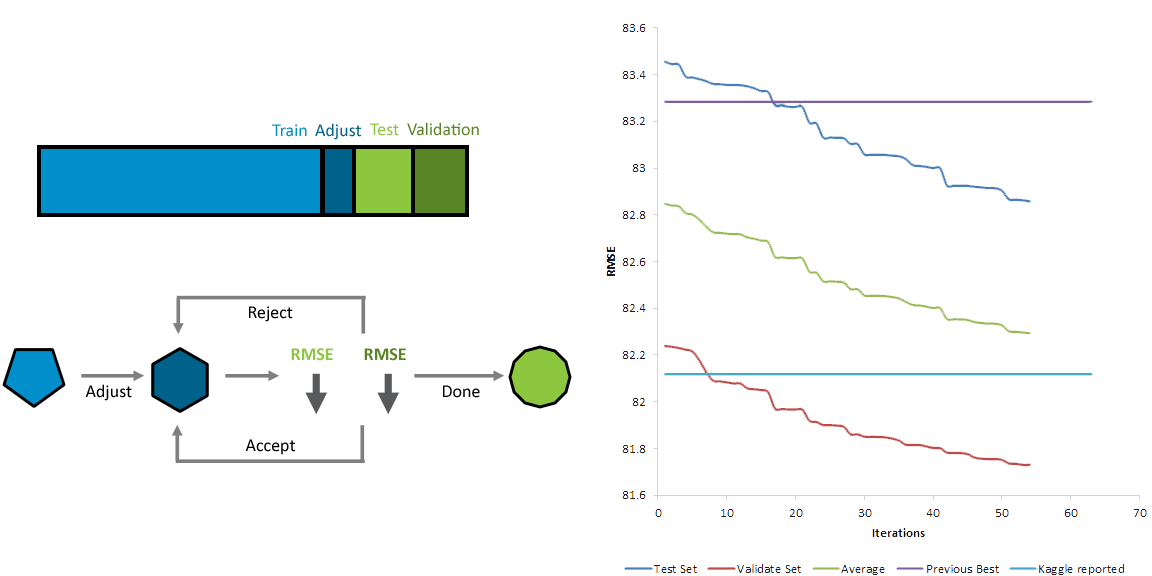
\includegraphics{expectedModelRefinement.png}}
	\end{center}
	\caption{(Left) Visual representation of refinement algorithm. (Right) RMSE as a function of algorithm iteration.}
	\label{fig:expectedValue:refinement}
\end{figure}

Finally, he automated this adjustment process as depicted in Fig. (\ref{fig:expectedValue:refinement}) by splitting the training set into four sets: two to initially fit and adjust the model, and two to verify adjustments reduced RMSE on two separate sets to mimic the Kaggle setup. An adjustment is applied to the model, if RMSE does not improve for both test sets, the adjustment is rejected, otherwise it is accepted, and the process continues until the adjustment set is exhausted. Result: RMSE of 82.11832 as our best Kaggle score until May 2\textsuperscript{nd}.

\section*{Right-Wrong Approach}

Tyler TODO (Sign, then position \& position then sign, features, error analysis)

\section*{Final Approach}

Alex TODO (Hedge bets, continuous yes/no sign prediction, features, error analysis)

\section*{Conclusions}

\paragraph{} Sunday we obtained our best score of 81.55246 based on the final approach. ...

\end{document}
